\chapter{Design}

To build a system capable of meeting the goals of the project it was important to design the system thoroughly from the start to ensure it would be easy to extend. To guarantee extendibility allowed for many different techniques to be quickly and effectively experimented on making the final system as accurate and as efficient as possible. This section discusses the various design decisions that were made, the reasoning behind the choices, and outlines the design of the final system that was used to meet the project objectives.

\section{What is an Error in a Tweet?}
Firstly, before any software was designed or written an important task was to define what an error is in the context of correcting spelling on Tweets. Of course, it is possible to define an error, simply, as a word or a phrase that doesn't exist in the English language. This definition would suffice in most contexts, such as general word processing, but this becomes far too simplistic when applied to such a specific problem like correcting the errors in Tweets from Twitter. Twitter has its own smaller subset of the English language while also including some of its own language features, such as contractions of words or Twitter keywords, therefore we must define errors based on this.

\begin{figure}[!h]
	\centering
	\label{fig:errorchart}
	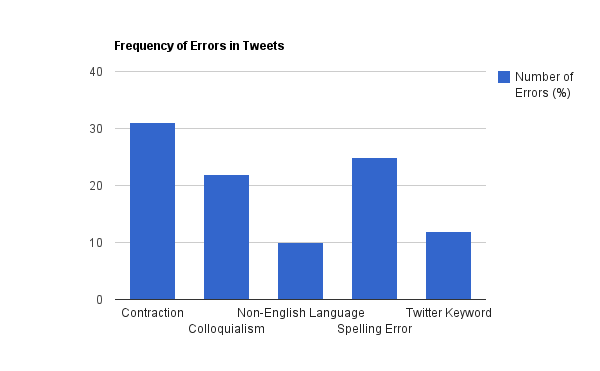
\includegraphics[scale=0.65]{images/errorfreqchart}
\end{figure}

To investigate the most common sources of errors in Tweets I corrected a set of Tweets with the Unix spelling error corrector Aspell. The results of my investigation are presented in figure \ref{fig:errorchart} above. From the investigation I found that over 30\% of errors that occurred were due to contractions. Contractions are a large part of the Twitter lexicon so it was important to take this into account before designing the system. As the system was to be used to correct spelling errors in Tweets for use in machine learning, where accuracy is key, I decided to attempt to correct contractions. As well as attempting to correct contractions I chose to keep statistics on the errors that occurred most often to indicate possible commonly used contractions. This collection of commonly used contractions could then, possibly, be filtered back into future executions to quickly and accurately correct contractions.

Another common source of spelling error in the Tweet dataset that is not a genuine spelling error is due to the language that the Tweet is written in. Twitter has a large number of users from all over the world and hence there are many Tweets that would contain many spelling errors when compared against an English dictionary. Although these words are technically spelling errors I decided that the system should not correct these as it would require a lot more computation and would slow the system down.

Finally, the last area of focus is the Twitter keyword. As explained in section 1.2 there are many Tweet specific keywords and features that will indicate a spelling error in generic spelling error detection software. Since the keywords are part of the language and may be important to future uses of the Twitter data I decided that whenever the system encounters an \emph{@username}, \emph{\#Hashtag}, \emph{RT}, or \emph{URL} it should ignore the error signal and continue correcting the rest of the Tweet.

\section{High-level System Design}
To build a system that meets all of the objectives set out at the beginning of the project a high-level system outline was created. The system required two main steps common to all spelling error detection and correction methods. These steps were:
\begin{itemize}
	\item
	loading and processing of the training texts;
	\item
	running the spelling error detection algorithm;
	\item
	ignoring words that shouldn't be corrected;
	\item
	running the error correction algorithms.
\end{itemize}

\section{Choosing the Error Correction Methods}
Selecting the error correction methods suitable for this task involved researching into prior work undertaken in the area of generic spelling correction. When searching for appropriate methods I took into account the accuracy of correction as well as the speed of correction. I felt that a good balance between accuracy and speed was required as some methods may perform better in terms of accuracy but take a lot more computational cycles which would hinder the overall effectiveness of a Twitter spelling error corrector that is required to run over terabytes of Tweets at a time.

Using the above criteria the Noisy Channel Method as described by Peter Norvig \cite{}, the character-level n-gram method as proposed by Ahmed et. al. \cite{}, and the context-sensitive n-gram method were selected. These methods were chosen as they represent a wide selection of the possible spelling error correction methods and have all been described as being effective on general spelling error correction. I also felt that it would be interesting to explore how the accuracy of the Tweet specific system compares to the results in general spelling error correction.

\section{Technologies}
One of the most important design decisions to make when designing a computer system is the language of implementation. Originally when building the first iteration of the system I decided upon choosing Java to implement the system. I made this initial decision as I have strong Java skills and the object-oriented nature of the language, particularly interfaces, fit well with the idea of being able to extend the system easily to add new features. Additionally, Java met the requirement of speed with its highly optimised virtual machine that has been refined over the years to produce an extremely efficient runtime environment. With respect to the data structures and methods required to implement each of the spelling error correction methods, Java includes an efficient key-value store called the HashMap and all of the string operations required.

Unfortunately, as implementation progressed it became increasingly cumbersome to implement the error correction methods with the verbosity of the Java language. For this reason I decided to rewrite the system into Python; another language that I was familiar with. Python's simplicity offered an increase in programming efficiency that allowed for more ideas to be experimented with. In addition, Python's string manipulation methods, particularly the ability to slice a string into arbitrary pieces, was incredibly useful. While Python has a much slower execution time than Java, the productivity gains were much more beneficial to the project.

With the switch to Python as the implementation language of choice it was also possible to introduce the Natural Language Toolkit (NLTK) \cite{} into the system. NLTK provides many common natural language functions that were useful in the implementation of the system, with the collocation finder and word tokeniser being of most use. This dramatically reduced the time to train the system as the functions are efficient and also more accurate than the naive algorithms that were first implemented in the Java version.

\section{Loading and Processing the Training Texts}
The first step in the Tweet spelling error corrector system is to load the training text and split them into their constituent words. To simplify later stages in the system, all words are stripped of any punctuation and converted to lower case to form a dictionary of accepted words. Once the words have been isolated a dictionary is formed by training the system on these words by simply counting the number of occurrences of each word found in the training texts and inserting them into a key-value store. This key-value store ensures constant-time, quick lookups to ensure efficiency. Words that occur less than 40 times are discounted from the dictionary in order to filter out any spelling errors in the training texts. The counts gained from this processing step are then saved to a file for use at a later time. By writing the values to a file this means that it is not necessary for subsequent executions of the correction system.

\section{Detecting Spelling Errors}
To detect errors in the Tweets the system performs a lookup on the provided dictionary for each word in the Tweet. The simple idea behind this method is that if the word is not in the dictionary, then it must be a spelling error.

Unfortunately this is too simplistic a view for a spelling error detection system as it must take into account the issues mentioned in section 2.1. To solve the first problem of language other than English being contained in Tweets I made the assumption that if more than half of the words in a Tweet are flagged as being spelled incorrectly then it is mostly likely that this Tweet is not English. For the Tweet-specific features such as \emph{@usernames} and \emph{\#Hashtags} I defined regular expressions to look for the patterns that the features exhibit. It is then possible to compare each word to the regular expression and if there is a match then that word can be ignored to save computational time and effort.

\section{Implementing the Noisy Channel Method}
The Noisy Channel method by Peter Norvig works by first generating all the possible ways that an error can be reversed into a correct word by a single edit operation. An edit operation can either be a deletion of one character, the insertion of one character, the replacement of one character by another, or the transposition of two adjacent characters. All of these possible edits are generated by simple string manipulation that does not require expensive computation.

Selecting the actual correction is then done by performing a lookup of each candidate correction in the key-value store and choosing the word with the highest probability based on the number of occurrences found in the training text.

\section{Implementing the Word-Level N-Gram Method}
\begin{itemize}
	\item Gather n-gram statistics
	\item Find possible corrections
	\item Rank based on context using n-gram statistics
\end{itemize}

\section{Implementing the Character-Level N-Gram Method}
To implement the character-level n-gram method, n-grams of size two (also known as bi-grams) were selected due to the fact that most spelling errors are caused by the mistyping of a single character. The bi-grams for the spelling error are calculated using string operations that select sub-strings of size two from the error. The set of bi-grams is then compared to each of the words in the key-value store by way of a n-gram similarity function which calculates the similarity between the error and a possible correction using equation 2. The correction method simply selects the word from the key-value store that is most similar to the error.

\section{Combining the Methods into a Voting Algorithm}
As an extension of the preceding algorithms I chose to combine all three spelling error correction algorithms into one combined algorithm. Voting algorithms are used in many applications in both Computer Science and other engineering fields to increase accuracy and reliability. The rationale behind using the algorithm is that by increasing the number of measurements the probability the system will produce an incorrect answer will decrease.

To actually implement a voting based system it is important to consider, firstly, how it will work and, secondly, how consensus will be reached in the result of a tie. The voting algorithm that I devised works by first asking each of the algorithms what their error correction would be if they were to correct the error in isolation. Each result of the algorithm represents a single vote in the voting algorithm. If there are two or more votes for one correction then a consensus has been reached and the correction returned by the system is simply this correction. As there three different voting algorithms it is possible that all three algorithms will disagree and a consensus cannot be reached. In the case of a stalemate a correction is chosen at random. The random choice is made as there is no way to decide whether one of the corrections is the most likely correct correction as each of the algorithms score their results differently and it might favour the algorithm that consistently gives a higher score.
